\documentclass[12pt]{article}
\usepackage[utf8]{inputenc}
\usepackage{amssymb,amsmath}
\usepackage{hyperref}
\usepackage{graphicx}
\usepackage{color}
\definecolor{gray}{gray}{.75}
\input{kvmacros}
\author{Claas Jaehrling, Sven-Hendrik Haase}
\title{RS1 HA zum 16.12.11}
\date{\today}
\begin{document}
\setcounter{secnumdepth}{0}
\maketitle

\section{Aufgabe 7.1}
\subsection{(a)}
\begin{align}
&Negation: \overline x = x \overline \lor x\\
&UND: x \land y = (x \overline \lor x) \overline \lor (y \overline \lor y)\\
&ODER: x \lor y = (x \overline \lor y) \overline \lor (x \overline \lor y)
\end{align}
\subsection{(b)}
\begin{align}
&f(x_3,x_2,x_1) = (\overline {x_3} \lor (x_2 \overline {x_1}))
(\overline {x_1} \lor (x_2 \overline {x_1})\\
&f_{NOR}(x_3,x_2,x_1) = ((x_3 \overline \lor x_3) \overline \lor 
(x_2 \overline \lor x_2 \overline \lor x_1)) \overline \lor x_1
\end{align}

\section{Aufgabe 7.2}


\section{Aufgabe 7.3}
\subsection{(a)}

\subsection{(b)}

\section{Aufgabe 7.4}
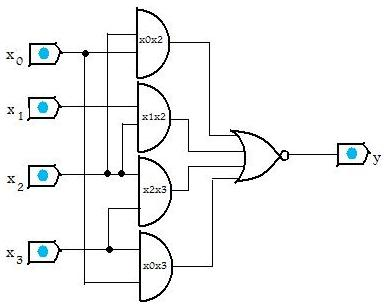
\includegraphics{Schaltnetz}
\subsection{(a)}
\begin{tabular} {rlll|l}
x0 & x1 & x2 & x3 & y \\ \hline 
0 & 0 & 0 & 0 & 0 \\
0 & 0 & 0 & 1 & 0 \\
0 & 0 & 1 & 0 & 0 \\
0 & 0 & 1 & 1 & 0 \\
0 & 1 & 0 & 0 & 0 \\
0 & 1 & 0 & 1 & 1 \\
0 & 1 & 1 & 0 & 0 \\
0 & 1 & 1 & 1 & 1 \\
1 & 0 & 0 & 0 & 0 \\
1 & 0 & 0 & 1 & 0 \\
1 & 0 & 1 & 0 & 0 \\
1 & 0 & 1 & 1 & 1 \\
1 & 1 & 0 & 0 & 1 \\
1 & 1 & 0 & 1 & 1 \\
1 & 1 & 1 & 0 & 1 \\
1 & 1 & 1 & 1 & 1
\end{tabular}

\subsection{(b)}
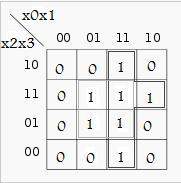
\includegraphics{KV-Diagramm1}

\subsection{(c)}
(siehe (b))\\
Schleife 1 (hellgrau):
\begin{align}
x_1 \land x_3
\end{align}
Schleife 2 (dunkelgrau):
\begin{align}
x_0((x_2 \land x_3) \lor x_1)
\end{align}
disjunktive Schaltfunktion:
\begin{align}
y = x_0 (x_2 x_3 \lor x_1) \lor x_1 x_3
\end{align}

\subsection{(d)}
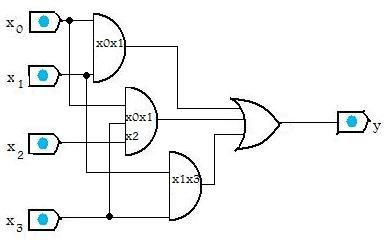
\includegraphics{Schaltplan}

\section{Aufgabe 7.5}

\subsection{(a)}
\begin{tabular} {r|rlll|l}
index & x0 & x1 & x2 & x3 & y \\ \hline 
    0 &  0 &  0 &  0 &  0 & 1 \\
    1 &  0 &  0 &  0 &  1 & 1 \\
    2 &  0 &  0 &  1 &  0 & 1 \\
    3 &  0 &  0 &  1 &  1 & 1 \\
    4 &  0 &  1 &  0 &  0 & 1 \\
    5 &  0 &  1 &  0 &  1 & 0 \\
    6 &  0 &  1 &  1 &  0 & 1 \\
    7 &  0 &  1 &  1 &  1 & 1 \\
    8 &  1 &  0 &  0 &  0 & 1 \\
    9 &  1 &  0 &  0 &  1 & 0 \\
   10 &  1 &  0 &  1 &  0 & 1 \\
   11 &  1 &  0 &  1 &  1 & 1 \\
   12 &  1 &  1 &  0 &  0 & 1 \\
   13 &  1 &  1 &  0 &  1 & 0 \\
   14 &  1 &  1 &  1 &  0 & 1 \\
   15 &  1 &  1 &  1 &  1 & 1
\end{tabular}

\karnaughmap{4}{f(x0,x1,x2,x3):}{{x0}{x1}{x2}{x3}}{1111101110111011}{}

\subsection{(b)}
Mögliche und sinnvolle Makrogruppen:\\
\karnaughmap{4}{f(x0,x1,x2,x3):}{{x0}{x1}{x2}{x3}}{1111101110111011}%
{%
\put(0,1){\colorbox{gray}{\makebox(3.8,2){}}}
}\\\\
\karnaughmap{4}{f(x0,x1,x2,x3):}{{x0}{x1}{x2}{x3}}{1111101110111011}%
{%
\put(0,0){\colorbox{gray}{\makebox(0.7,4){}}}
\put(3,0){\colorbox{gray}{\makebox(0.7,4){}}}
}\\\\
\karnaughmap{4}{f(x0,x1,x2,x3):}{{x0}{x1}{x2}{x3}}{1111101110111011}%
{%
\put(0,2){\colorbox{gray}{\makebox(1.7,1.7){}}}
}\\

disjunktive Schaltfunktion:
\begin{align}
y = x2 \lor \overline {x3} \lor \overline {x0x1}
\end{align}

\end{document}
